\chapter{Methodology}\label{ch:methodology}

The problem described in the previous chapter can be summarized in one sentence:

\begin{quote}
\begin{center}
\emph{Is it possible to build a model able to capture the topics or concepts commonly addressed when talking or writing about musical beauty?}
\end{center}
\end{quote}

As a first step towards finding an answer to this question, we will take advantage of well studied \acsfont{NLP} techniques and apply them to a collection of music reviews\footnote{Using \acsfont{NLP} techniques, such as word embeddings, to disentangle complex semantic concepts has been attempted before. One such example can be found in \cite{rodda2016panta}, where the authors managed to automatically identify the areas of
semantic change in the lexicon of Ancient Greek between the pre-Christian and Christian
era.}. The path we will follow for doing so is to obtain a structured representation of the words contained in such reviews, so that mathematical properties of the resulting \emph{semantic spaces}\footnote{While no formal definition of semantic spaces exist, a common understanding is that it is a topological space made up of words or concepts that are connected by certain relationships (\cite{masucci2011wikipedia}).} can be exploited to uncover existing semantic relationships between the modeled terms. By querying this model with input words closely related to beauty, we will obtain a set of words which, according to the model's internal representation, are the most semantically related to the input. Finally, we will try to classify the returned similar words, to check whether recurring topics will emerge.

The first phase consisted of gathering the required data. In the following section, I am thus going to describe the adopted dataset.

\section{A dataset of Pitchfork album reviews}
Pitchfork\footnote{\url{https://pitchfork.com/}} is a music-centric online magazine, launched in 1995 by Ryan Schreiber and currently based in Chicago, Illinois. It grew out of independent music reviewing into a general publication format. According to the company\footnote{See \cite{pitchfork}}, the website receives <<[...] more than 7 million monthly unique visitors>>.

For our research we will start from a collection of 18\,393 Pitchfork album reviews that have been previously scraped from the web and made openly accessible on the Kaggle platform\footnote{\url{https://www.kaggle.com/nolanbconaway/pitchfork-data}}. The collected reviews span an 18-years period, with the earliest having been published on the 5th of January, 1999, and the most recent on the 8th of January, 2017. Reviews were written by 432 different reviewers.

The albums reviewed belong to 8\,633 different artists, and each album has been reviewed only once. An album is characterized by zero, one or more genre labels, as summarized in \autoref{tab:genres}.

\begin{table}[t]
    \myfloatalign
    \begin{tabular}{lc}
        \toprule
        \tableheadline{Genre} & \tableheadline{Albums}\\
        \midrule
        rock 			& 9\,436 \\
        electronic 	& 3\,874 \\
        experimental	& 1\,815 \\
        rap			& 1\,559 \\
        pop/r\&b 		& 1\,432 \\
        \bottomrule
    \end{tabular}
    \begin{tabular}{lc} 
        \toprule
        \tableheadline{Genre} & \tableheadline{Albums}\\
        \midrule
        metal 		& 860 \\
        folk/country 	& 685 \\
        jazz 			& 435 \\
        global 		& 217 \\
        \emph{<unlabeled>}	& 2\,367 \\
        \bottomrule
    \end{tabular}
    \caption[Genre labels of the reviewed albums]{Genre labels of the reviewed albums. The \emph{genre} column indicates the label of the genre; the \emph{albums} column indicates the number of albums associated with that label.}
    \label{tab:genres}
\end{table}

Additional pieces of information provided by the dataset include the score given by the reviewer to an album (on a scale from 0 to 10), the record label under which the album has been published, and the content itself of the review, which constitutes the most relevant bit of data for our purposes.

\section{Word embeddings}
What we have at disposal is thus an extended collection of documents, in free-text form, from which we wish to extract the closest terms to some input set of words related with beauty. This list will be introduced in \autoref{sec:query}. For doing so, we first have to represent the words contained in the documents in a way that allows us to easily compute distances between terms in an unsupervised manner (i.e., without human intervention). The most suitable approaches to achieve this involve using the so-called \emph{word embeddings}.

Under the umbrella name ``word embeddings'' are included a variety of \acsfont{NLP} techniques aimed at mapping words -- or in some cases even entire sentences -- from a vocabulary onto vectors of real numbers. In mathematical language, we can define a word embedding in the following way:
$$
V \rightarrow \mathbb{R}^D : w \mapsto \vec{w}
$$
meaning a word embedding is a mapping that maps a word $w$ from a vocabulary $V$ to a real-valued vector $\vec{w}$ in an embedding space of dimensionality $D$. In the simplest case, the vocabulary would be built from the collection of all the single words used in the reviews taken only once.

In order to achieve this task, we have focused our attention on two classes of models. The first one is based on \emph{co-occurrence matrices}, while the second one is known as \emph{word2vec}.

\subsection{Co-occurrence matrices}\label{subsec:coocc}
A co-occurrence matrix is a simple data structure in a matrix form holding how many times any term appears in the same context with every other term in the vocabulary. Contexts are defined as a small number of words surrounding the target word, as entire paragraphs, or even as documents (\cite{pado2007dependency}). The assumption is that the more often two terms appear in the same context, the more similar their vector form is, and, consequentially, the more similar they are according to the model. \cite{font2013folksonomy}, for example, have taken advantages of these peculiar types of matrices to build a tag recommendation system for sound collections.

To compute the co-occurrence matrix, first we need to build a \emph{bag-of-words} (\acsfont{BOW}) representation of the words of the vocabulary. A bag-of-words is defined as a matrix $\mathbf{A}$ of size $M \times N$, where $M$ is the number of documents in our collection, and $N$ is the number of terms in our vocabulary. The element $a_{m,n}$ of the matrix holds how many times the term $n$ appears in the document $m$. The similarity matrix $\mathbf{S}$ based on term-term co-occurrence is then the result of the multiplication of the document-term matrix $\mathbf{A}$ by its transposed form:
$$
\mathbf{S} = \mathbf{A}\mathbf{A}^\mathsf{T}
$$

Each row of $\mathbf{S}$ can be seen as a multidimensional vector representing word $n$, defined in function of its co-occurrence with all the other words in the vocabulary. As such, we can obtain a single similarity value between any two words by computing the \emph{cosine similarity} of their representative vectors $\mathbf{s}$ and $\mathbf{t}$:
\begin{equation} \label{eq:cossim}
\text{similarity} = 
{\mathbf{s} \cdot \mathbf{t} \over \|\mathbf{s}\| \|\mathbf{t}\|} = 
\frac
{ \sum\limits_{i=1}^{n}{\mathbf{s}_i \mathbf{t}_i} }
{ \sqrt{\sum\limits_{i=1}^{n}{\mathbf{s}_i^2}} \sqrt{\sum\limits_{i=1}^{n}{\mathbf{t}_i^2}} }
\end{equation}

Cosine similarity can vary between 0 and 1, where 0 indicates that the two word vectors are completely dissimilar, and 1 that the two word vectors are the same.

Semantic and syntactic relationships generated in this way can be quite powerful; unfortunately, the drawbacks of applying it on such a big corpus pose serious limits, preventing us from adopting it on the totality of our data. In fact, given the high number of documents and the size of the vocabulary (more than 300\,000 unique words), $\mathbf{S}$ results in an enormous sparse matrix of more than 90 \emph{billion} entries. While preprocessing the text can partially help\footnote{During this phase we applied standard stop-words removal and stemming.}, the amount of information to process is still too demanding in terms of both time and, most importantly, memory.

There exist more advanced techniques that build on top of co-occurrence matrices, such as \emph{latent semantic analysis} and its probabilistic variation (\acsfont{LSA} and \acsfont{PLSA} respectively, see \cite{hofmann1999probabilistic}), but we will not adopt them for the same reasons outlined above.

\subsection{Word2vec}
Word2vec is a collection of two related models for computing continuous vector representations of words from very large datasets. They have been presented and further refinished in \cite{mikolov2013distributed} and \cite{mikolov2013efficient}. The architecture of both models consists of a shallow neural network with a single hidden layer. What we are interested in are the weights learned by this hidden layer once the training of the model has been completed\footnote{In \cite{vijayakumar2017sound}, for example, a word2vec model has been successfully trained to learn word representations grounded in sound.}.

The difference between the two models of word2vec lies in the way they compute the hidden layer. The first model, called \emph{continuous bag-of-words} (\acsfont{CBOW}), aims at predicting a target word by looking at its context words, whereas the second model, called \emph{Skip-gram}, follows the inverse path: given the target word, it will try to predict its context\footnote{We can define context words as the words to the left and to the right of our target word. A \emph{window size} hyperparameter will tell the model how many context words should be taken into account during the training process.}.

According to \citeauthor{mikolov2013efficient}, \acsfont{CBOW} performs better and faster with larger amounts of data; Skip-gram is better suited when the size of the dataset is smaller, and when the amount of rare words is bigger. For these reasons, we chose to adopt the latter model. Even though the amount of words contained in our corpus is notable (more than 12.6 million terms\footnote{Note that the amount of terms in the corpus and the size of the vocabulary mentioned in \autoref{subsec:coocc} are different, since in the vocabulary we only account for unique words.}), word2vec is known to produce meaningful results only when the size of corpora is in the order of tens of millions words upwards. In other words, the size of our dataset is barely enough.

Input layer and output layer both consist of $W$ neurons, where $W$ is the number of
words in the vocabulary of the given text corpus. The hidden input layer consists of $n$ neurons, where $n$ is another hyperparameter of the model and defines the dimensionality of the vector representation of each word we wish to obtain. \autoref{fig:skipgram} illustrates a dummy example of a Skip-gram model while it is being trained on predicting the context of the word ``ant''.

\begin{figure}[bth]
	\myfloatalign
	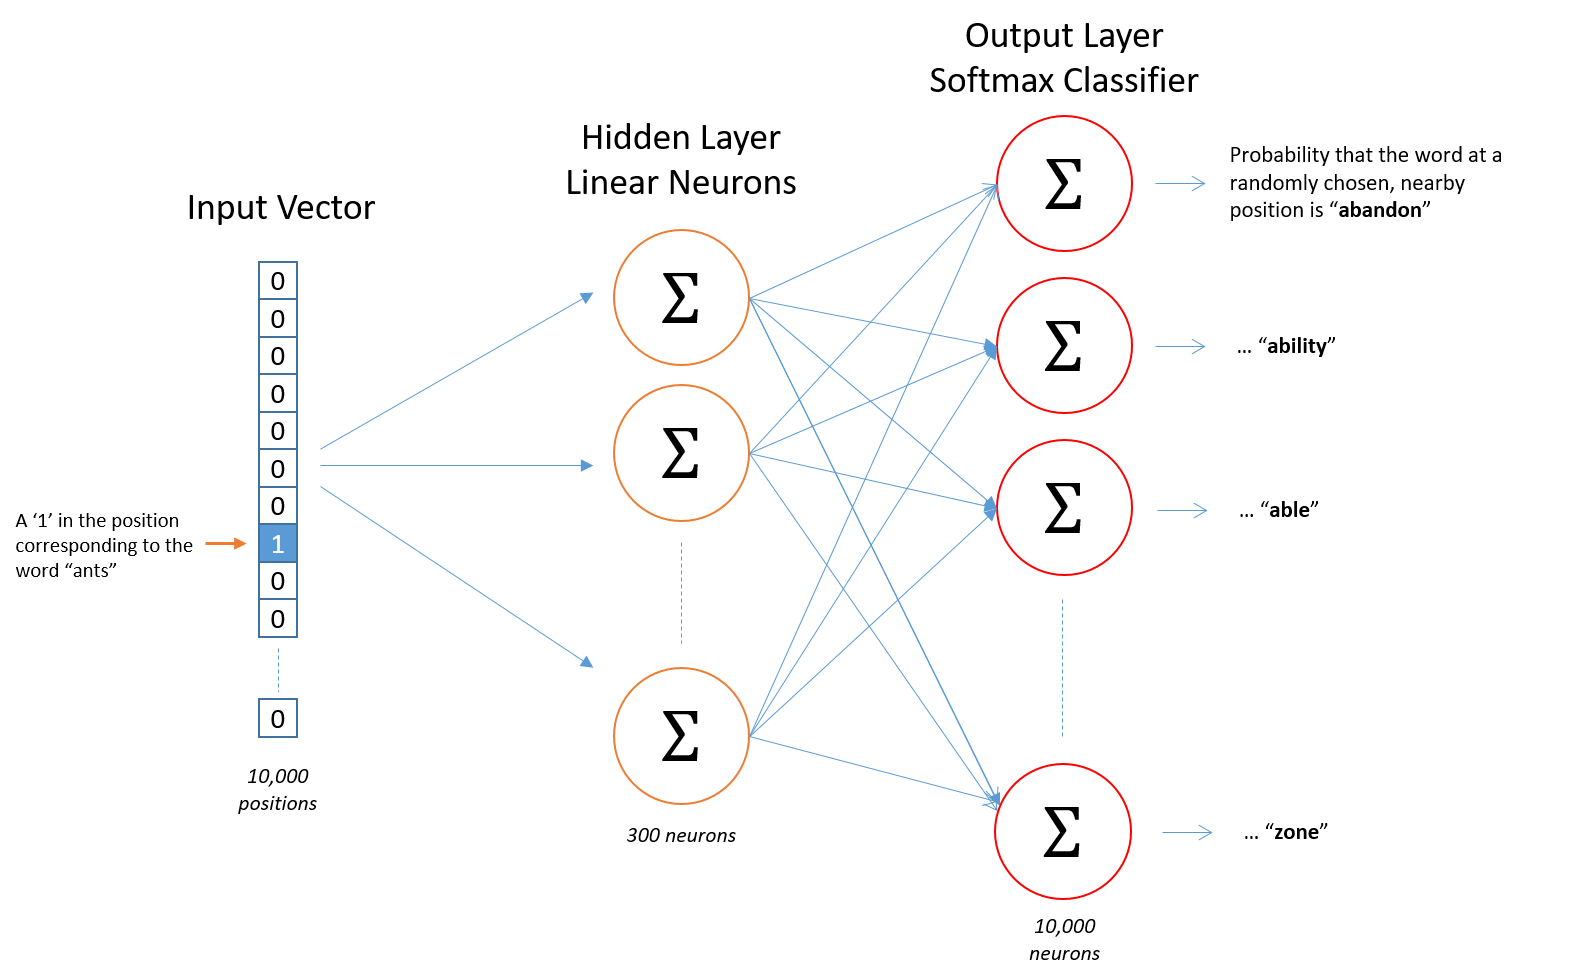
\includegraphics[width=\linewidth]{gfx/word2vec_arch}
	\caption[Architecture of a word2vec skip-gram model]{Example of a Skip-gram architecture. We can observe that $W = 10\,000$ and $n = 300$, meaning \emph{(a)} that the input vocabulary contains 10\,000 terms, and \emph{(b)} that for every word we wish to obtain a 300-dimensional vector representation. Here, the hyperparameter defining the window size is not shown.}
	\label{fig:skipgram}
\end{figure}

The input layer (also called \emph{projection layer}) receives words as a \emph{one hot encoded} vector, i.e. a vector of length $v$ where each element is equal to 0, except for the element whose position corresponds to the position of the input word in the vocabulary. If the vocabulary contains 10\,000 words, and the word ``ant'' appears in it at position 8, the input vector will contain all zeroes, and a single 1 in the 8th element.

A more formal definition of the Skip-gram model is as follows. Given a sequence of words $w_1, w_2, w_3, \dots, w_T$, i.e. the words in our vocabulary, the objective of the model is to maximize the average log probability, defined as:

\begin{equation} \label{eq:logprob}
\frac{1}{T} \sum\limits_{t=1}^{T}
\sum\limits_{-c \leq j \leq c, j \neq 0}
\log p(w_{t+j}|w_t)
\end{equation}
where $c$ is the window size. Skip-gram ideally defines $p(w_{t+j}|w_t)$ using a \emph{softmax} function:
\begin{equation} \label{eq:softmax}
p(w_O|w_I) = 
\frac
{\exp\left({\mathbf{v}'}_{w_O} {}^\mathsf{T} \mathbf{v}_{w_I}\right)}
{\sum\limits_{w=1}^{W}\exp\left({\mathbf{v}'}_w {}^\mathsf{T} \mathbf{v}_{w_I}\right)}
\end{equation}
where $\mathbf{v}_w$ and $\mathbf{v}'_w$ are the input and output vector representations of the word $w$, and $W$ is the number of words in the vocabulary.

However, this formulation is quite expensive, because its computing cost is proportional to the number $W$ of words in the vocabulary (which, in our case, we know to be around 300\,000). \citeauthor{mikolov2013efficient}, in order to approximate the full softmax\footnote{The first version of word2vec uses another approximation of the softmax, the \emph{hierarchical softmax}, not discussed here.}, propose a more efficient method, the \emph{negative sampling} (\acsfont{NEG}). \acsfont{NEG} is defined by the following objective function, which will replace every $\log P(w_O|w_I)$ term in \autoref{eq:logprob}:
\begin{equation} \label{eq:negsamp}
\log \sigma\left(\mathbf{v}'_{w_O} {}^\mathsf{T} \mathbf{v}_{w_I}\right) +
\sum\limits_{i=1}^k \mathbb{E}_{w_i \sim P_n(w)}
\left[\log \sigma\left(-\mathbf{v}'_{w_i} {}^\mathsf{T} \mathbf{v}_{w_I}\right)\right]
\end{equation}

Here, $\sigma(x) = 1 / (1 + \exp(-x))$. The task of this optimization is to distinguish the target word $w_O$ from random draws from the noise distribution $P_n(w)$ using logistic regression. The hyperparameter $k$ defines the \emph{negative samples}, or how many words from the noise distribution will be chosen to be ``distinguished'' from the target word $w_O$. The noise distribution $P_n(w)$ has been set by the authors as
$$
\frac{U(w)^{3/4}}{Z}
$$
where $U(w)$ is the \emph{unigram distribution}. The reported value in their experiments has been observed to outperform both the simple unigram distribution and the uniform distribution.

A perhaps more intuitive explanation of the Skip-gram architecture with negative sampling is the following. Whenever the model receives an input word $w_I$ as a one hot encoded vector $\mathbf{h}$, it retrieves from the projection layer the neuron $\mathbf{n}_i$, where $i$ is the index of the only element equal to 1 in $\mathbf{h}$ (the position of the word inside the vocabulary). This neuron holds the weights of the vector representation of $w_I$. Note that before the training starts, each neuron in the projection layer has to be initialized, usually with small random values.

In an ideal scenario (i.e., when using softmax, see \autoref{eq:softmax}), during training each vector representation of all the words $w_O$ in the vocabulary should either be ``pulled closer'' to $\mathbf{n}_i$ or ``pushed away'' from $\mathbf{n}_i$ by a small fraction, depending respectively on whether $w_O$ belongs to the context of $w_I$ or not. With negative sampling, however, the operation of ``pushing away'' the out-of-context word vectors is not performed for every word in the vocabulary, but only on a small subset randomly chosen from all of the out-of-context words.

There is a further optimization worth mentioning, due to the fact that it will affect data preprocessing. Raw textual sources contain a high number of words which do not carry much information, such as articles and prepositions. For example, if the model will benefit from observing the co-occurrence of the term ``guitarist'' with the term ``guitar'', it will benefit much less from observing the co-occurrence of the term ``the'' with the term ``guitarist'', since almost every word can co-occur frequently with ``the'' in a sentence. For this reason, Skip-gram subsamples frequent words according to the following equation:
\begin{equation}
P(w_i) = 1 - \sqrt{\frac{t}{f(w_i)}}
\end{equation}
meaning that each word $w_i$ in the training set will be discarded with a probability $P(w_i)$. The term $f(w_i)$ is the frequency of the word $w_i$, and $t$ is an arbitray threshold, set by the authors at around $10^{-5}$.

The advantages of adopting the Skip-gram model are several: 
\begin{itemize}
\item we can perform a \emph{streamed} type of training, meaning that less computational resources are needed since we won't have to keep all of the corpus loaded in memory all the time; in fact, we can feed the model with one sentence at a time, and then discard it when the next sentence comes in.
\item supposing the generated vector representations contain 300 elements each\footnote{This is an indicative value most people tend to suggest as an upper limit, after which overfitting will likely occur, but the choice of the vector size depends on the application.}, the output matrix computed on our vocabulary will only contain about 90 million entries, corresponding to 0.1\% of the size of what we would get by using simple co-occurrence matrices;
\item the amount of needed preprocessing is minimal, because, as we have seen, Skip-gram already contemplates a mechanism for discarding irrelevant terms; moreover, processes such as stemming\footnote{Stemming is the process of reducing inflected (or sometimes derived) words to their word stem, base or root form (e.g., the words ``beauty'', ``beautiful'' and ``beautifully'' share the same word stem ``beauti'').} and lemmatization\footnote{Lemmatization is the process of grouping together the inflected forms of a word so they can be analysed as a single item, identified by the word's lemma, or dictionary form (e.g., the words ``play'', ``plays'' and ``played'' share the same lemma ``play'').} become less relevant, because the model should implicitly figure out that terms sharing the same stem or lemma are in some way similar.
\end{itemize}

This said, the main reason supporting our choice of relying on this model is that the resulting vector representations will not only generate a semantic space where similar words end up close to each other, but they will be able to represent multiple degrees of similarity between words (\cite{mikolov2013linguistic}). For our purpose, and given the difficulties encountered in attributing to aesthetic terminology a universal meaning, we could maybe expect to observe one of two scenarios: words such as ``beauty'' or ``beautiful'' will \emph{(a)} be very similar to many different (musical) categories of terms (belonging to emotions, instruments, genres, \ldots), or \emph{(b)} live in a rather isolated corner of the output semantic space, distant from any specific/recognizable category of items.

\subsubsection{Preprocessing and training}
Before training the model, it is necessary to build the vocabulary we wish to represent. It has been said before that usually the vocabulary of a dataset is the collection of the single terms used in the documents; however, \citeauthor{mikolov2013efficient} suggest to include in the vocabulary idiomatic phrases whose meaning does not derive from a simple composition of the individual words -- what in technical language are referred to as \emph{n-grams}. Examples of music inspired n-grams would be ``electric guitar'', or ``hip hop'', or ``Guns'n'Roses''. Therefore, we first generated a list of n-grams (up to phrases of three words, or trigrams\footnote{N-grams can make the model more expressive, but they will also increase data sparsity, so we should be careful and use them with care.}) taken from our corpus that were added to the vocabulary.

Once we defined a vocabulary, we finally trained the Skip-gram model on a lowercased copy of the dataset. Lowercasing raw text is a common preprocessing step in \acsfont{NLP} tasks aimed at data cleaning (e.g., words appearing at the beginning of a sentence, or typos). The hyperparameters used in the training are reported in \autoref{tab:hyper}.
\begin{table}[t]
	\myfloatalign
	\begin{tabularx}{\textwidth}{lXc}
	\toprule
	\tableheadline{Parameter} & \tableheadline{Description} & \tableheadline{Value} \\
	\midrule
	size		& Size of each word's vector representations & 300 \\
	window 	& Maximum distance between the current word and the predicted context words within a sentence & 5 \\ 
	negative & Number of negative samples & 5 \\
	\bottomrule
	\end{tabularx}
	\caption{Hyperparameters of the word2vec Skip-gram model}
	\label{tab:hyper}
\end{table}

\section{Querying and clustering}\label{sec:query}
Any word embedding will generate a semantic space, a high-dimen\-sional projection of the vocabulary where every word is represented by vectors. These vectors can be seen as points occupying a specific position inside this multidimensional space. As such, we can apply standard clustering techniques to further describe the semantic space, and to characterize the similarities between words. If it is possible to succesfully cluster together words that appear to share a semantic connection, it means that there are good chances the embedding contains organized information, for which the clustering itself can provide some degree of explanation\footnote{In the next chapter, a less hand-wavy method for evaluating the quality of a word embedding will be introduced, along with results obtained on our dataset.}.

For this task, what we did was to query the Skip-gram model trained on our data with a list of ``aesthetic terms'', in order to obtain the closest words to each input query. This simple list comprises the following groups of words:
\begin{itemize}
	\item aesthetic -- aesthetics
	\item beautiful -- beautifully -- beauty
	\item ugliness -- ugly
\end{itemize}
which are very explicit terms related to aesthetics or to beauty (along with their antonyms, adjectives and adverbs).

We finally used a k-means algorithm to cluster the ``close terms'', or \emph{nearest neighbours}, returned from the model. The nearest neighbours of a word $w$ are all words $v \in V \setminus \left\{w\right\}$ (where $V$ is the vocabulary) sorted in descending order by $\text{similarity}(w,v)$; the similarity, again, is defined by the cosine distance between vector representations of $w$ and $v$ (see \autoref{eq:cossim}). By doing so we tried to identify semantic classes of word clusters that could reasonably answer our question: what do people refer to when they argue over musical beauty?

\section{Final note}
All the code and the data used in the steps reported here and in the next chapter are open-source and accessible at the following link:
\begin{quote}
	\url{https://github.com/lorenzo-romanelli/compbeauty_code}
\end{quote}
























